% !TeX spellcheck = en_US

\chapter{Supporting Information on the Screening Study}
\label{ap:screening}

\begin{figure*}
	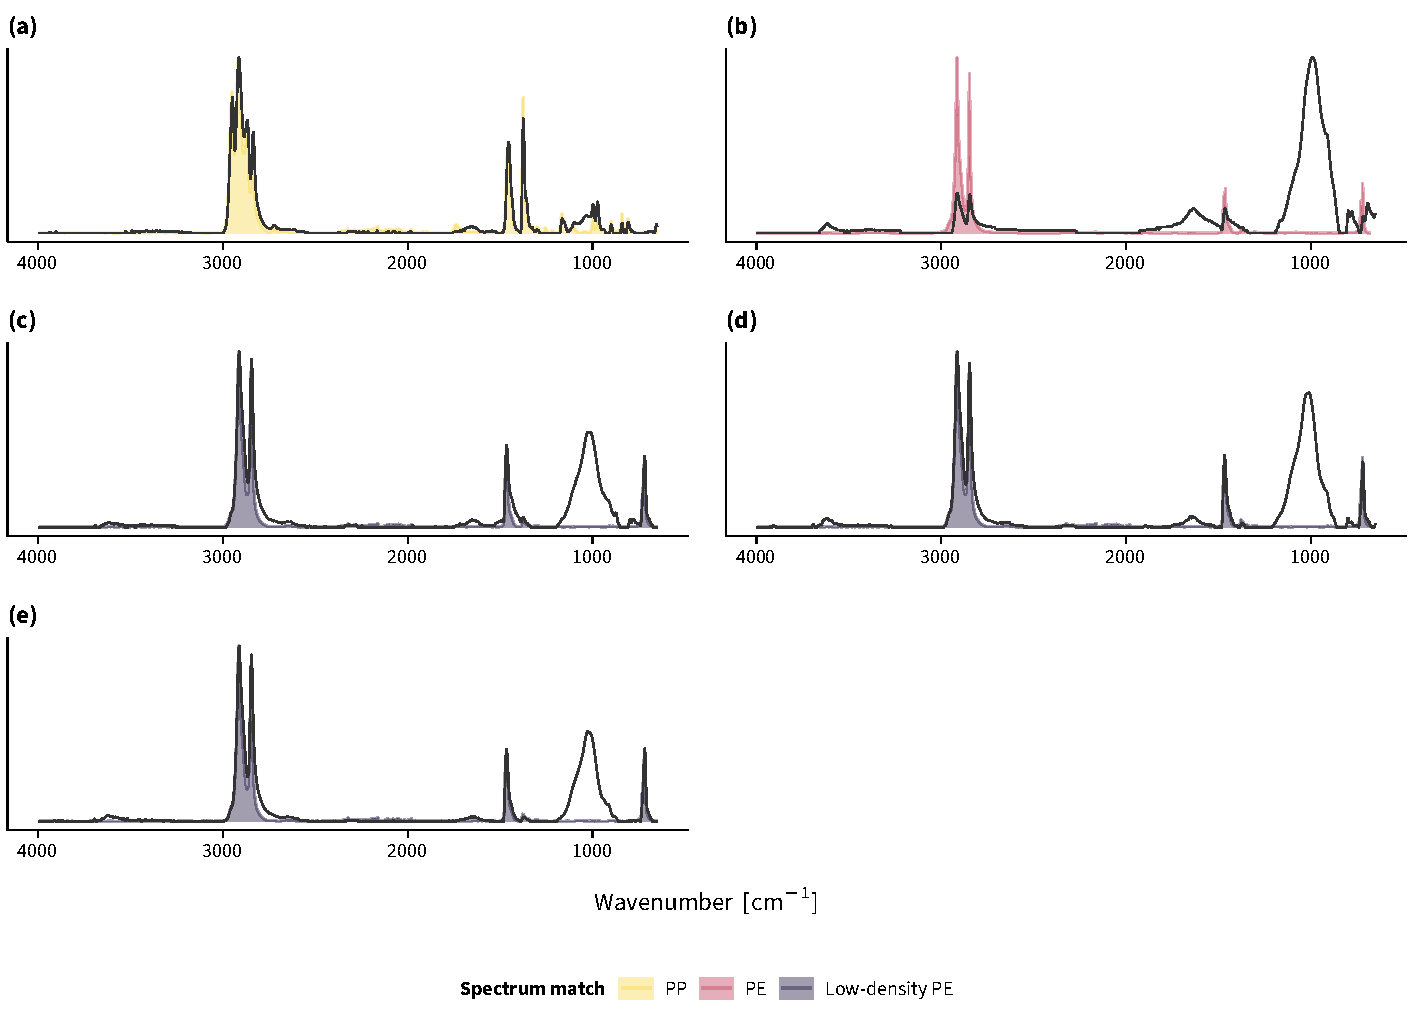
\includegraphics[width=\textwidth]{figures/ftir-covers}
	\caption[Exemplary \ac{ftir} spectra of the agricultural plastic covers on site.]{Exemplary \ac{ftir} spectra of (a) the \ac{pp} fleece from site 1, (b) the \ac{pe} mulch from sites 2 and 3, (c) the \ac{pe} fleece and (d) \ac{pe} perforated foil from sites 4 and 5, and (e) the \ac{pe} perforated foil from site 8. The measured \ac{ftir} spectra are in gray; the colored shades depict the respective Open Specy library match.}
	\label{fig:ftir-covers}
\end{figure*}

\begin{figure*}
	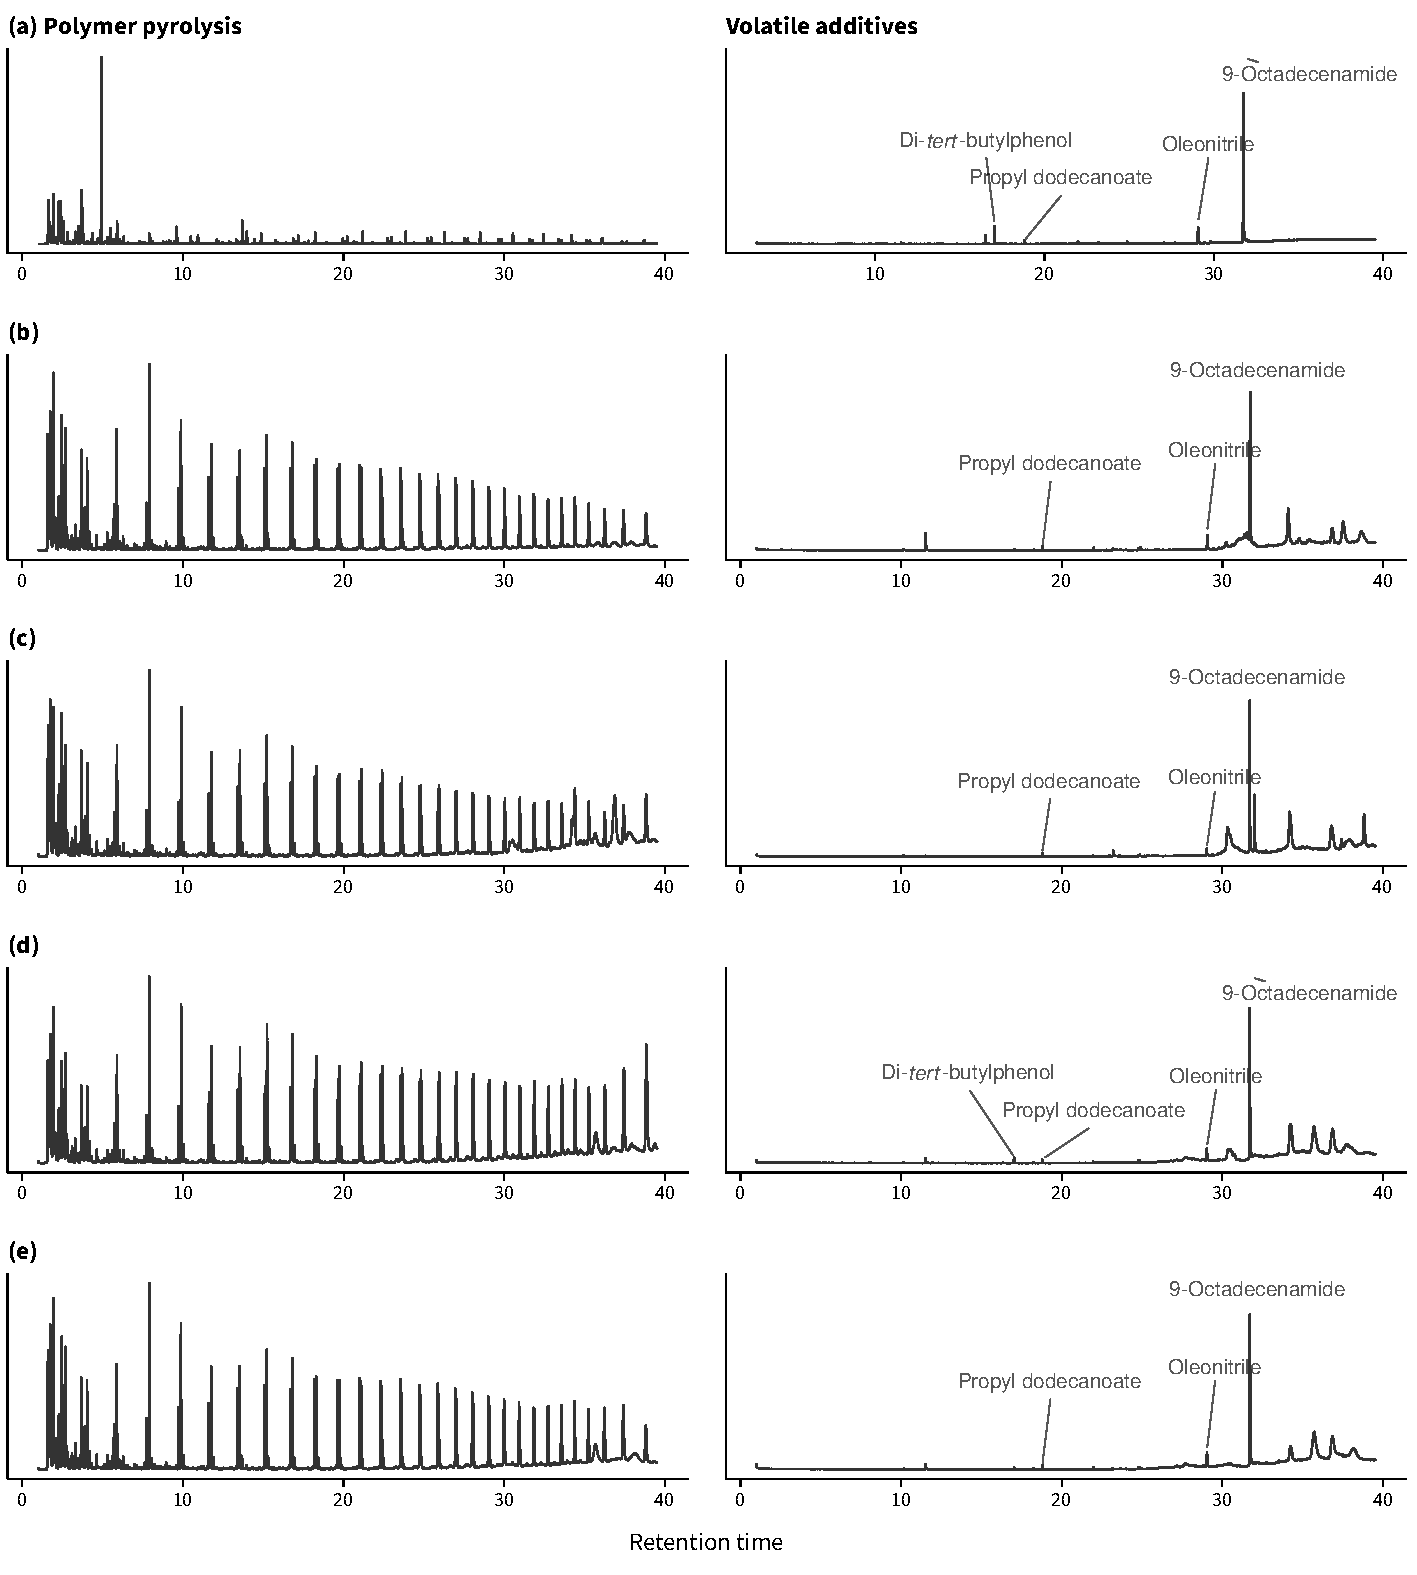
\includegraphics[width=\textwidth]{figures/py-covers}
	\caption[Exemplary chromatograms of polymer pyrolyses and thermal desorptions of polymer additives of the agricultural plastic covers.]{Exemplary chromatograms of polymer pyrolyses (\SI{750}{\degreeCelsius}, left) and thermal desorptions (\SI{300}{\degreeCelsius}, right) of polymer additives; (a) \ac{pp} fleece from site 1, (b) \ac{pe} mulch from sites 2 and 3, (c) \ac{pe} fleece and (d) \ac{pe} perforated foil from sites 4 and 5, and (e) \ac{pe} perforated foil from site 8; see Figure~\protect\ref{fig:ms-covers} for mass spectra.}
	\label{fig:py-covers}
	\forceversofloat
\end{figure*}

\begin{figure*}[p]
	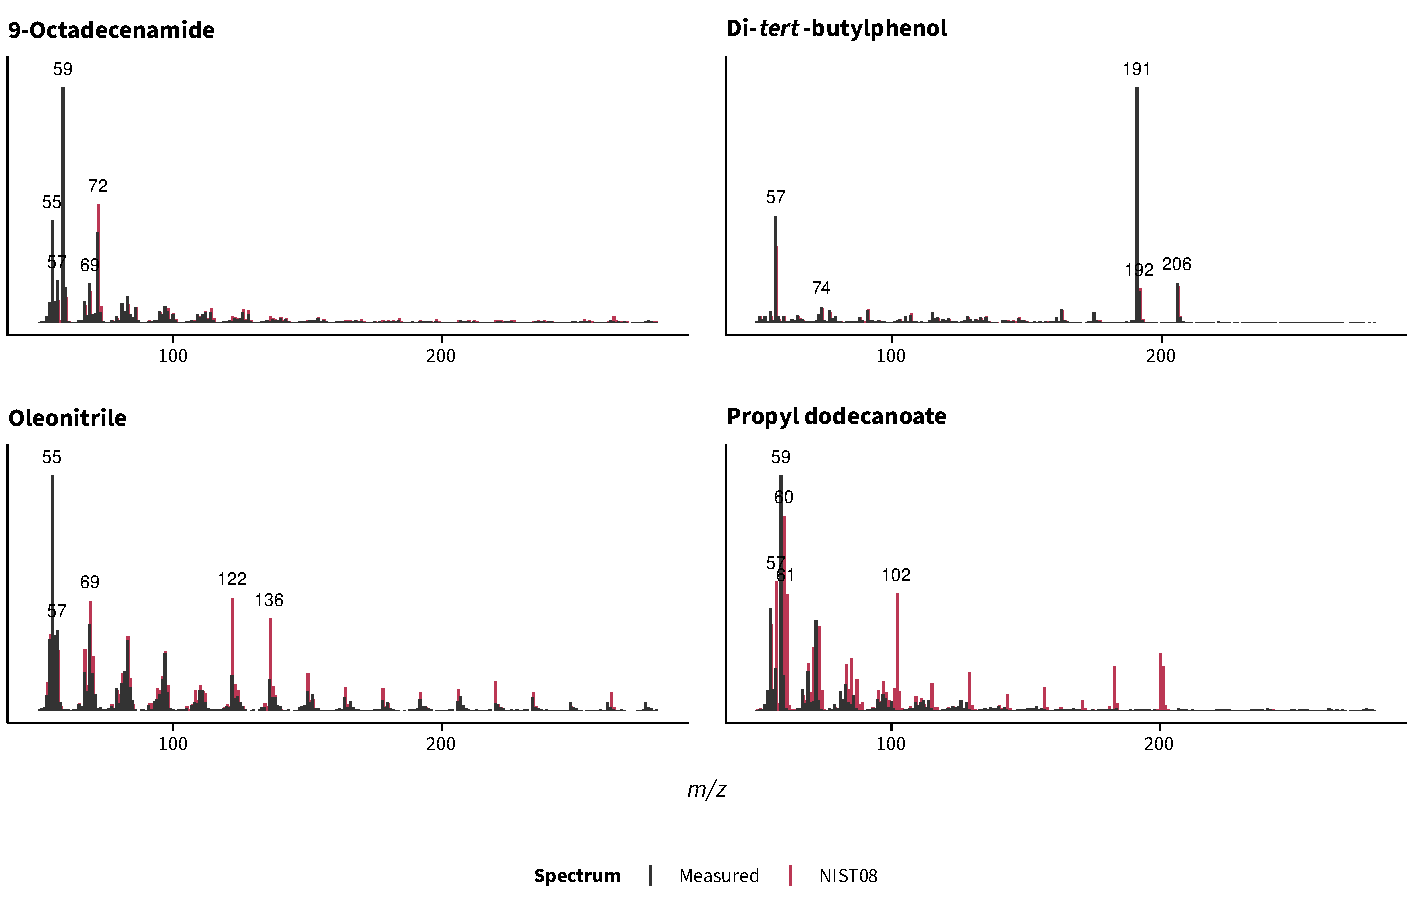
\includegraphics[width=\textwidth]{figures/ms-covers}
	\caption[Mass spectra and NIST08 library matches of the identified polymer additives.]{Mass spectra and NIST08 library matches of the identified polymer additives that thermally desorbed from the agricultural films; see Figure~\protect\ref{fig:py-covers} for chromatograms.}
	\label{fig:ms-covers}
\end{figure*}

\clearpage

\begin{figure*}[p]
	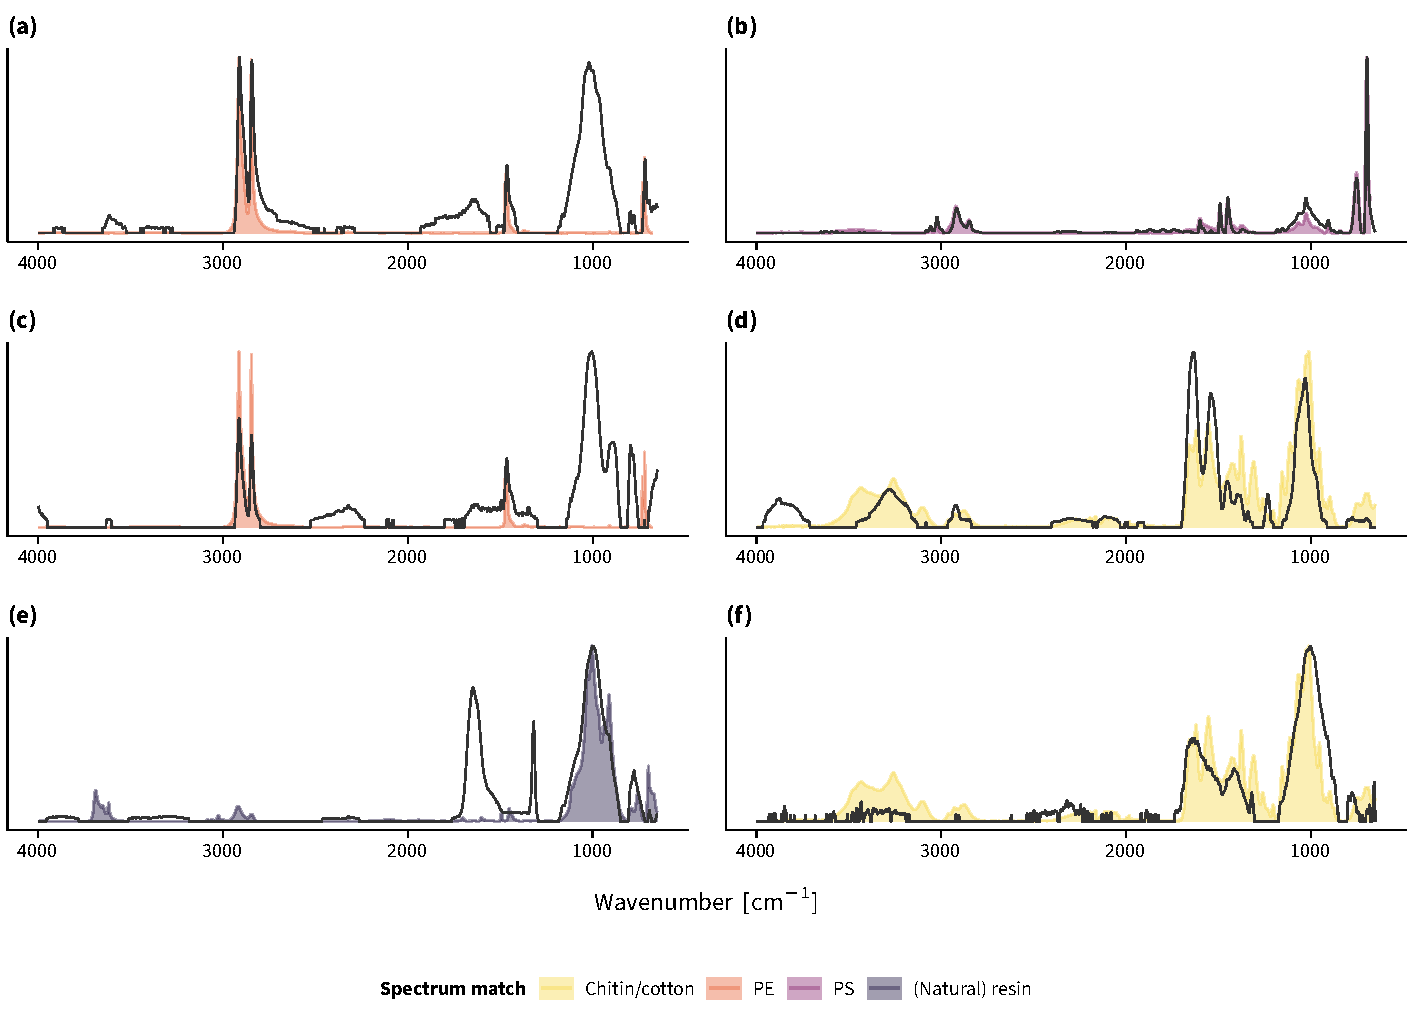
\includegraphics[width=\textwidth]{figures/ftir-debris}
	\caption[\Ac{ftir} spectra of the debris shown in Figure~\protect\ref{fig:visual-items}.]{\Ac{ftir} spectra of the debris shown in Figure~\protect\ref{fig:visual-items}; (a) \ac{pe} film and (b) \ac{ps} fragment from the field center of site 5, (c) \ac{pe} film and (d) chitin shell from the field center of site 6, and (e) resin or natural fragment and (f) cotton fiber from the field edge of site 7. The measured \ac{ftir} spectra are in gray; the colored shades depict the respective Open Specy library match.}
	\label{fig:ftir-debris}
\end{figure*}

\clearpage

\begin{figure*}[p]
	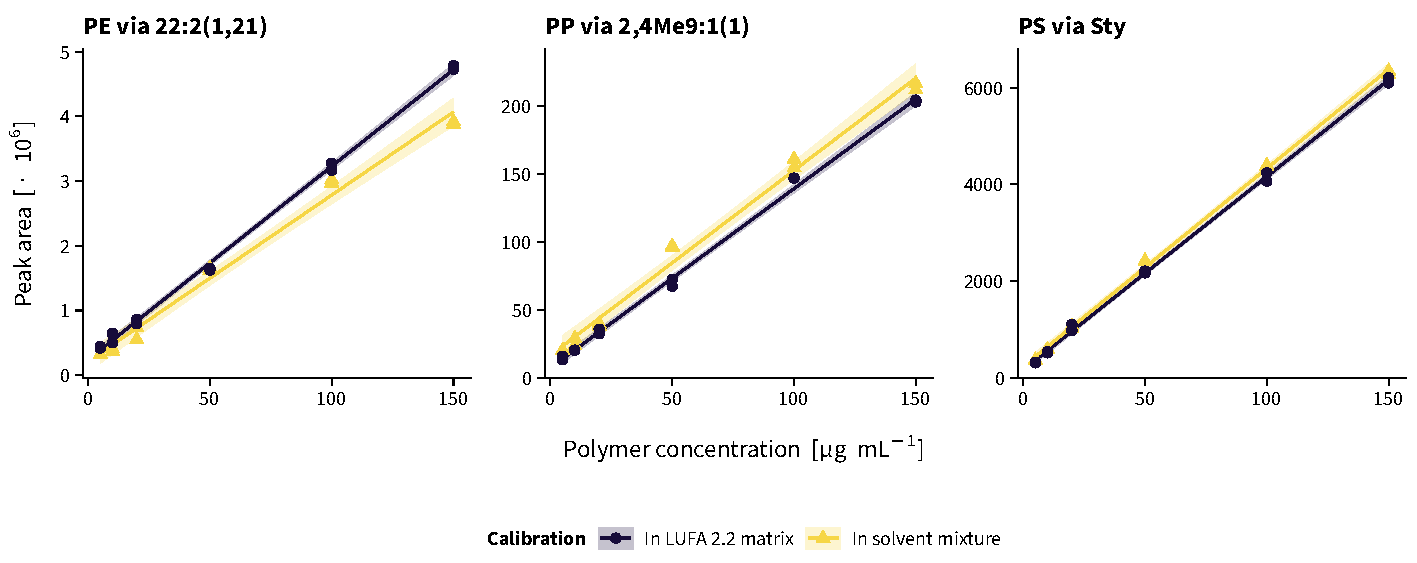
\includegraphics[width=\textwidth]{figures/matrix-match}
	\caption{\Ac{py-gc-ms} calibration in solvent \textit{p}-xylene/\ac{tcb} and in LUFA 2.2 matrix compared.}
	\label{fig:matrix-match}
	\forcerectofloat
\end{figure*}
